\subsection{Gateway}
This section we will be detailing our plans for incorporating a LoRaWAN gateway into our design. We will not be designing the hardware in the same way that we are designing the hardware for the sensor node i.e. designing the PCB, etc., but we will need to build a functioning LoRaWAN gateway in order for sensor node to be useful. This section will focus on what we will need to do to set up the physical gateway components, which are a Raspberry Pi 4 and a RAK 2245 Pi Hat. We will also discuss how the software will need to be set up on the gateway in order to be able to connect it to our AWS instance, The Things Network, and The Helium Network.

\subsubsection{Gateway Hardware}
The hardware assembly for the gateway is incredibly simple. All that needs to be done is to attach the RAK 2245's connector to the Raspberry Pi's 40-pin GPIO header. After this, it is simply a matter of connecting the Ethernet output to an internet router and plugging in the micro-USB cable for power. Additionally, the GPS antenna and the LoRa antenna that come with the RAK 2245 must be attached to it in order for the gateway to function. The only other component that is required is an SD card loaded with a Linux image developed by RAKWireless designed for the gateway. Our setup gateway can be seen is Figure \ref{fig:gateway-rak}.

\begin{figure}
    \centering
    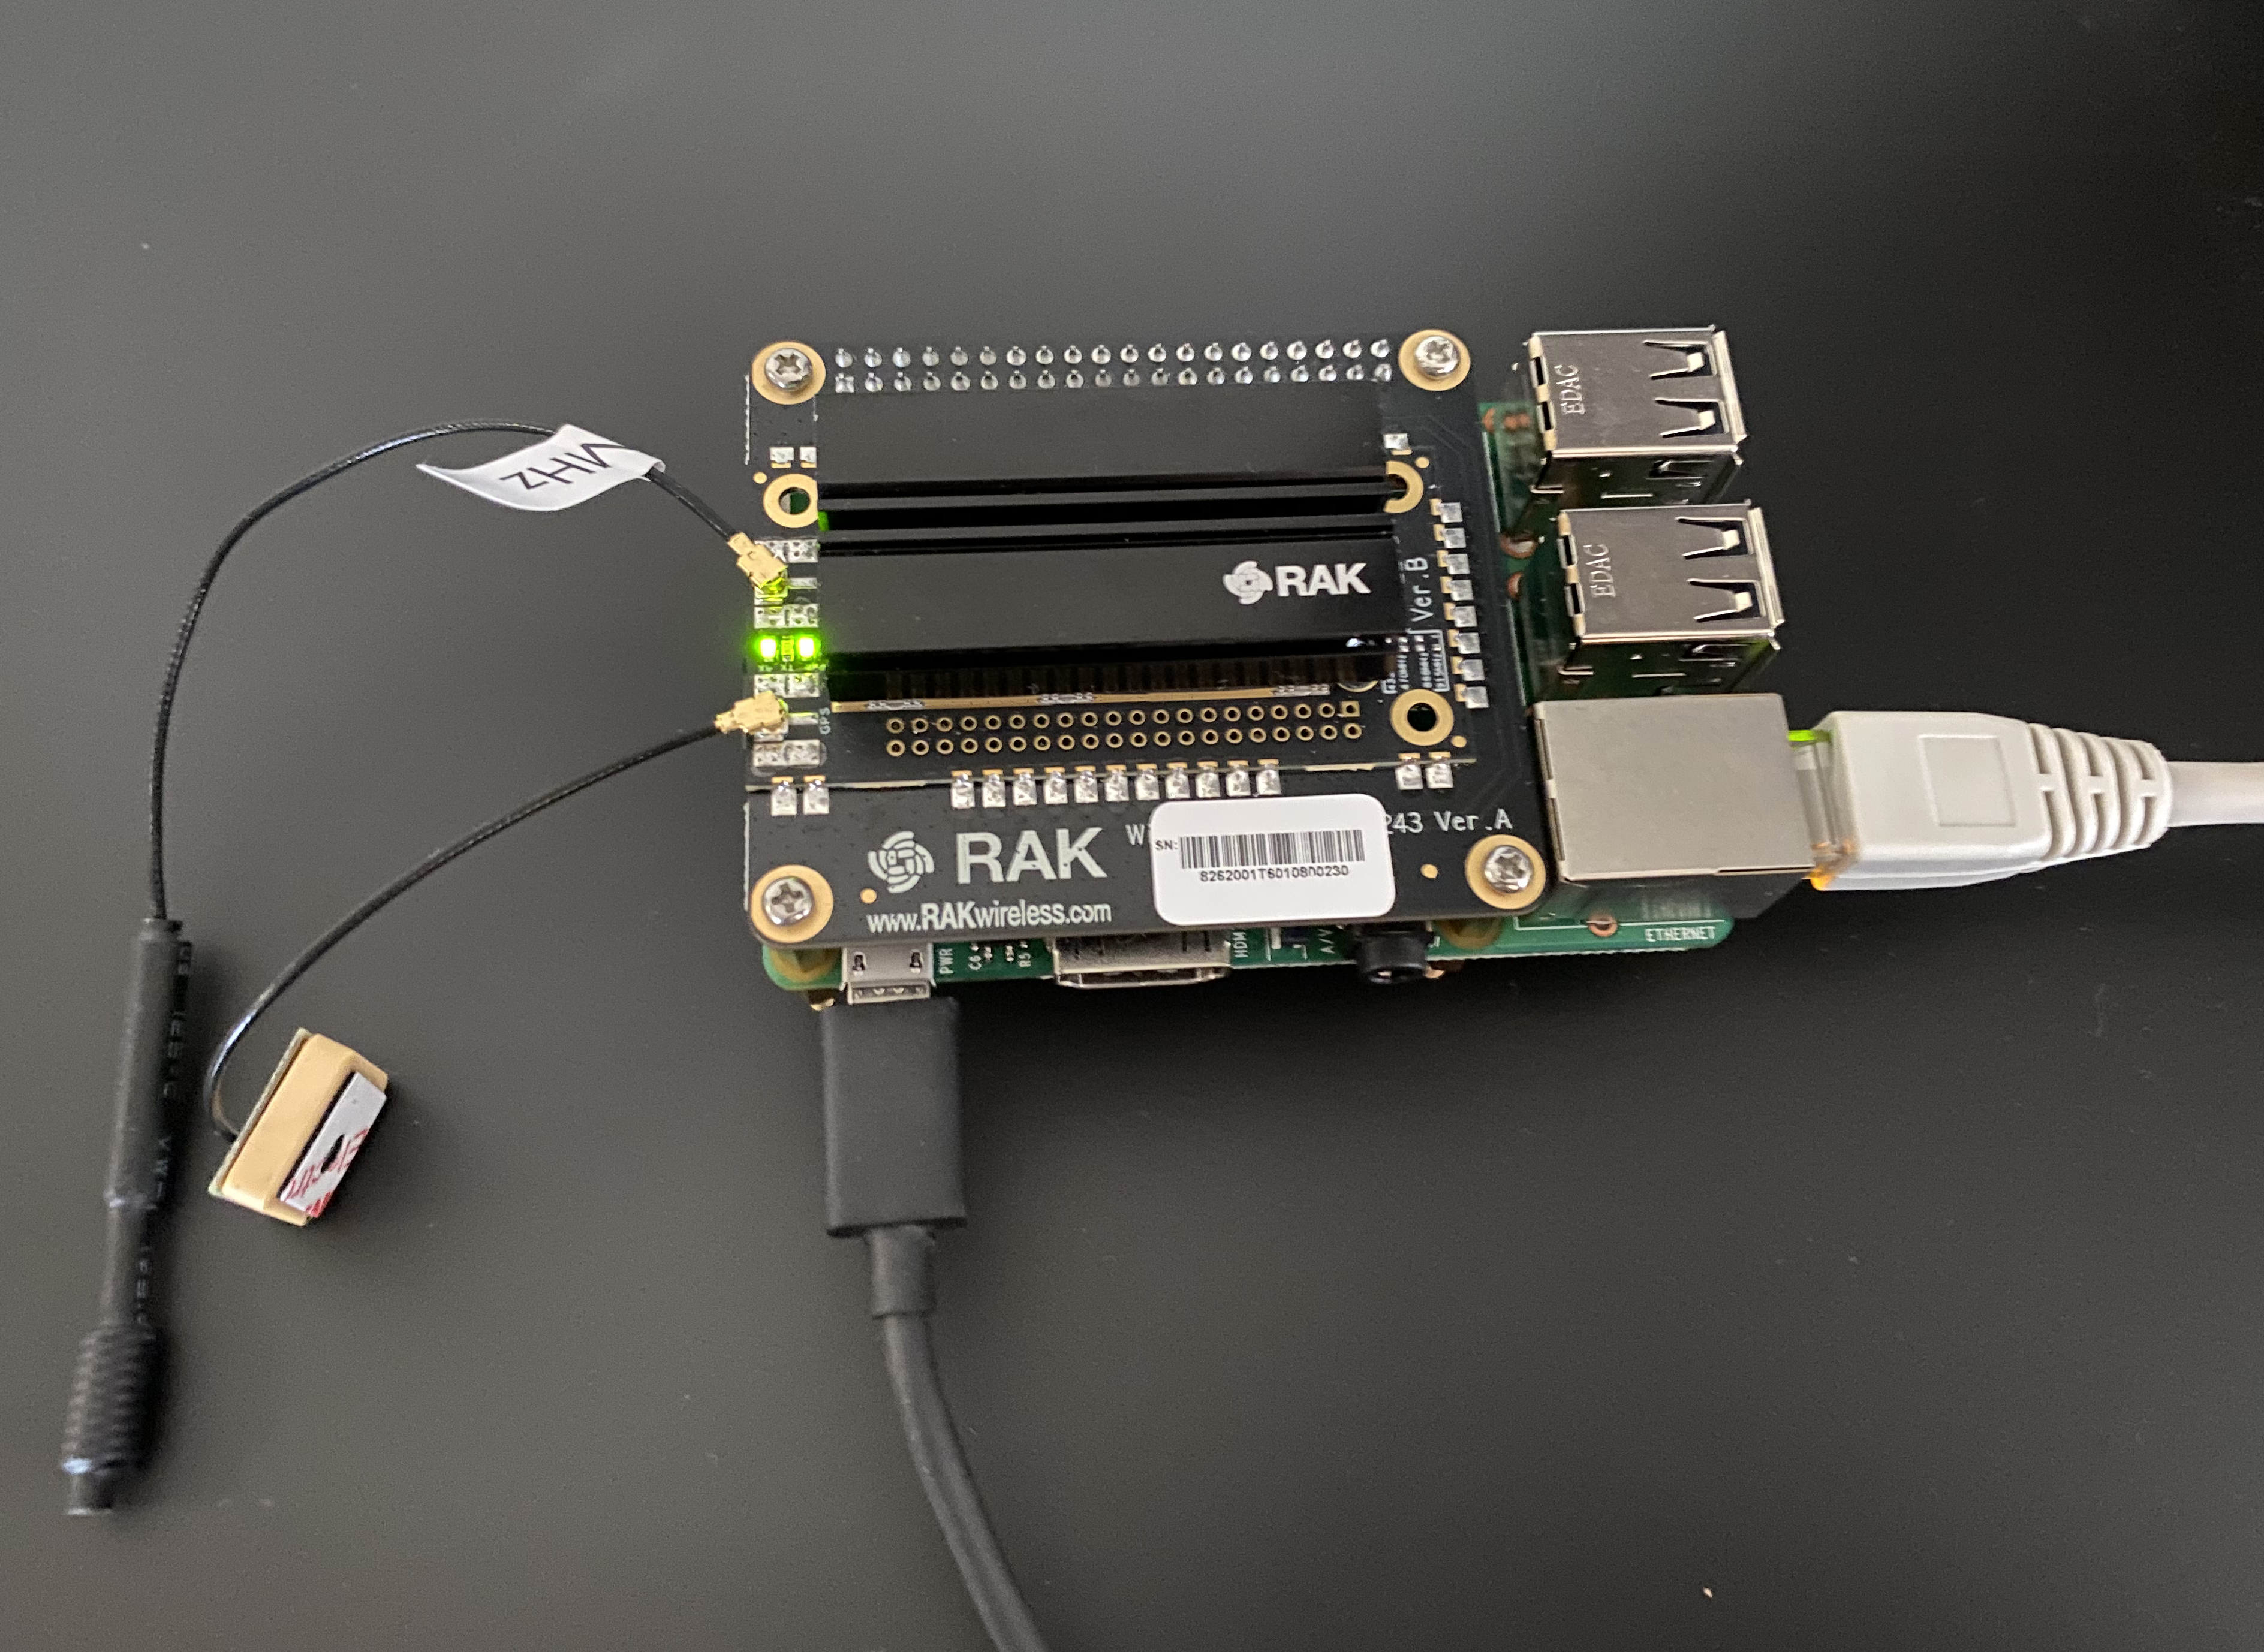
\includegraphics[width=4.5in]{figures/gateway-rak.png}
    \caption{An image of our setup gateway. It shows the Raspberry Pi 4 connected with the RAK 2245 Pi Hat.}
    \label{fig:gateway-rak} 
\end{figure}

\subsubsection{Gateway Software}
Configuring the gateway to function with the various LoRaWAN networks we desire is also fairly straightforward. Once we burn the previously mentioned OS image to an SD card and insert it into the Raspberry Pi, the device will create a new WiFi access point. On a separate computer, we will be able to connect to this WiFi access point and then can gain access to the gateway via an SSH connection. Within this SSH connection is where we will be able to configure that gateway to connect to any of the LoRaWAN networks we choose. In the next few sections we will detail how we will connect our gateway to The Things Network, The Helium Network, and directly to our AWS server instance.

\paragraph{Connecting to The Things Network}
Connecting to The Things Network is simply a matter of configuring the LoRaWAN gateway and using The Things Network's online configuration tool to add your gateway to the network.

To configure the gateway itself, one needs to connect to the gateway via SSH and then run the \texttt{gateway-config} command as follows. Also, run the \texttt{gateway-version} command. The information from this command will be used to add the gateway to the network.

\begin{tabular}{l}
     \texttt{\$ ssh pi@192.168.10.10} \\
     \texttt{\$ sudo gateway-config} \\
     \texttt{\$ sudo gateway-version} \\ 
\end{tabular}

This will bring up a menu GUI. In this menu, you select option 2, "\texttt{Setup RAK Gateway LoRa concentrator}. Then select the server plan, which is \texttt{Server is TTN}. Next, you select the appropriate region and frequency region, which in our case is \texttt{US\_902\_928}. After this, configuration on the device itself is finished. We will need to move to the Things Network's website next.

To finish setting up our gateway with The Things Network, we must navigate to The Things Network's website\footnote{The website for The Things Network is \texttt{www.thethingsnetwork.org}} and create an account. Once logged in, navigate to the Console, select your region, and then click "Add gateway." Once there, fill out the appropriate information for the gateway including the \texttt{Gateway ID} and appropriate frequency plan. After completing this, any LoRaWAN end-device that is correctly configured to connect to The Things Network should be able to see your newly setup gateway and use it to connect to the internet.

\paragraph{The Helium Network}

\paragraph{Connecting Our AWS Server Instance}

